\subsection*{试题背景}

{\heiti{动态主机配置协议}}(Dynamic Host Configuration Protocol, DHCP)是一种自动为网络客户端分配 IP 地址的网络协议。当支持该协议的计算机刚刚接入网络时,它可以启动一个 DHCP 客户端程序。后者可以通过一定的网络报文交互,从 DHCP 服务器上获得 IP 地址等网络配置参数,从而能够在用户不干预的情况下,自动完成对计算机的网络设置,方便用户连接网络。DHCP 协议的工作过程如下:

\begin{enumerate}

    \item 当 DHCP 协议启动的时候,DHCP 客户端向网络中广播发送 Discover 报文,请求 IP 地址配置;

    \item 当 DHCP 服务器收到 Discover 报文时,DHCP 服务器根据报文中的参数选择一个尚未分配的 IP 地址,分配给该客户端。DHCP 服务器用 Offer 报文将这个信息传达给客户端;

    \item 客户端收集收到的 Offer 报文。由于网络中可能存在多于一个 DHCP 服务器,因此客户端可能收集到多个 Offer 报文。客户端从这些报文中选择一个,并向网络中广播 Request 报文,表示选择这个 DHCP 服务器发送的配置;

    \item DHCP 服务器收到 Request 报文后,首先判断该客户端是否选择本服务器分配的地址:如果不是,则在本服务器上解除对那个 IP 地址的占用;否则则再次确认分配的地址有效,并向客户端发送 Ack 报文,表示确认配置有效,Ack 报文中包括配置的有效时间。如果 DHCP 发现分配的地址无效,则返回 Nak 报文;

    \item 客户端收到 Ack 报文后,确认服务器分配的地址有效,即确认服务器分配的地址未被其它客户端占用,则完成网络配置,同时记录配置的有效时间,出于简化的目的,我们不考虑被占用的情况。若客户端收到 Nak 报文,则从步骤 1 重新开始;

    \item 客户端在到达配置的有效时间前,再次向 DHCP 服务器发送 Request 报文,表示希望延长 IP 地址的有效期。DHCP 服务器按照步骤 4 确定是否延长,客户端按照步骤 5 处理后续的配置;

\end{enumerate}

在本题目中,你需要理解 DHCP 协议的工作过程,并按照题目的要求实现一个简单的 DHCP 服务器。


\subsection*{问题描述}

\subsubsection*{报文格式}

为了便于实现,我们简化地规定 DHCP 数据报文的格式如下:

\begin{lstlisting}
<发送主机> <接收主机> <报文类型> <IP 地址> <过期时刻>
\end{lstlisting}

DHCP 数据报文的各个部分由空格分隔,其各个部分的定义如下:

\begin{itemize}

    \item 发送主机:是发送报文的主机名,{\heiti{主机名}}是由小写字母、数字组成的字符串,唯一地表示了一个主机;

    \item 接收主机:当有特定的接收主机时,是接收报文的主机名;当没有特定的接收主机时,为一个星号(\verb|*|);

    \item 报文类型:是三个大写字母,取值如下:\begin{itemize}

              \item \verb|DIS|:表示 Discover 报文;

              \item \verb|OFR|:表示 Offer 报文;

              \item \verb|REQ|:表示 Request 报文;

              \item \verb|ACK|:表示 Ack 报文;

              \item \verb|NAK|:表示 Nak 报文;

          \end{itemize}



    \item IP 地址,是一个非负整数:\begin{itemize}

              \item 对于 Discover 报文,该部分在发送的时候为 0,在接收的时候忽略;

              \item 对于其它报文,为正整数,表示一个 IP 地址;

          \end{itemize}



    \item 过期时刻,是一个非负整数:\begin{itemize}

              \item 对于 Offer、Ack 报文,是一个正整数,表示服务器授予客户端的 IP 地址的过期时刻;

              \item 对于 Discover、Request 报文,若为正整数,表示客户端期望服务器授予的过期时刻;

              \item 对于其它报文,该部分在发送的时候为 0,在接收的时候忽略。

          \end{itemize}



\end{itemize}

例如下列都是合法的 DHCP 数据报文:

\begin{lstlisting}
a * DIS 0 0
d a ACK 50 1000
\end{lstlisting}

\subsubsection*{服务器配置}

为了 DHCP 服务器能够正确分配 IP 地址,DHCP 需要接受如下配置:

\begin{itemize}

    \item 地址池大小 $N$:表示能够分配给客户端的 IP 地址的数目,且能分配的 IP 地址是 $1, 2, \dots, N$;

    \item 默认过期时间 $T_{def}$:表示分配给客户端的 IP 地址的默认的过期时间长度;

    \item 过期时间的上限和下限 $T_{max}$、$T_{min}$:表示分配给客户端的 IP 地址的最长过期时间长度和最短过期时间长度,客户端不能请求比这个更长或更短的过期时间;

    \item 本机名称 $H$:表示运行 DHCP 服务器的主机名。

\end{itemize}

\subsubsection*{分配策略}

当客户端请求 IP 地址时,首先检查此前是否给该客户端分配过 IP 地址,且该 IP 地址在此后没有被分配给其它客户端。如果是这样的情况,则直接将 IP 地址分配给它,否则,
总是分配给它最小的尚未占用过的那个 IP 地址。如果这样的地址不存在,则分配给它最小的此时未被占用的那个 IP 地址。如果这样的地址也不存在,说明地址池已经分配完毕,因此拒绝分配地址。

\subsubsection*{实现细节}

在 DHCP 启动时,首先初始化 IP 地址池,将所有地址设置状态为未分配,占用者为空,并清零过期时刻。
其中地址的状态有未分配、待分配、占用、过期四种。
处于未分配状态的 IP 地址没有占用者,而其余三种状态的 IP 地址均有一名占用者。
处于待分配和占用状态的 IP 地址拥有一个大于零的过期时刻。在到达该过期时刻时,若该地址的状态是待分配,则该地址的状态会自动变为未分配,且占用者清空,过期时刻清零;否则该地址的状态会由占用自动变为过期,且过期时刻清零。处于未分配和过期状态的 IP 地址过期时刻为零,即没有过期时刻。

对于收到的报文,设其收到的时刻为 $t$。处理细节如下:

\begin{enumerate}

    \item 判断接收主机是否为本机,或者为 \verb|*|,若不是,则判断类型是否为 Request,若不是,则不处理;

    \item 若类型不是 Discover、Request 之一,则不处理;

    \item 若接收主机为 \verb|*|,但类型不是 Discover,或接收主机是本机,但类型是 Discover,则不处理。

\end{enumerate}

对于 Discover 报文,按照下述方法处理:

\begin{enumerate}

    \item 检查是否有占用者为发送主机的 IP 地址:\begin{itemize}

              \item 若有,则选取该 IP 地址;

              \item 若没有,则选取最小的状态为未分配的 IP 地址;

              \item 若没有,则选取最小的状态为过期的 IP 地址;

              \item 若没有,则不处理该报文,处理结束;

          \end{itemize}



    \item 将该 IP 地址状态设置为待分配,占用者设置为发送主机;

    \item 若报文中过期时刻为 0 ,则设置过期时刻为 $t + T_{def}$;否则根据报文中的过期时刻和收到报文的时刻计算过期时间,判断是否超过上下限:若没有超过,则设置过期时刻为报文中的过期时刻;否则则根据超限情况设置为允许的最早或最晚的过期时刻;

    \item 向发送主机发送 Offer 报文,其中,IP 地址为选定的 IP 地址,过期时刻为所设定的过期时刻。

\end{enumerate}

对于 Request 报文,按照下述方法处理:

\begin{enumerate}

    \item 检查接收主机是否为本机:\begin{itemize}

              \item 若不是,则找到占用者为发送主机的所有 IP 地址,对于其中状态为待分配的,将其状态设置为未分配,并清空其占用者,清零其过期时刻,处理结束;

          \end{itemize}



    \item 检查报文中的 IP 地址是否在地址池内,且其占用者为发送主机,若不是,则向发送主机发送 Nak 报文,处理结束;

    \item 无论该 IP 地址的状态为何,将该 IP 地址的状态设置为占用;

    \item 与 Discover 报文相同的方法,设置 IP 地址的过期时刻;

    \item 向发送主机发送 Ack 报文。

\end{enumerate}

上述处理过程中,地址池中地址的状态的变化可以概括为如下图所示的状态转移图。为了简洁,该图中没有涵盖需要回复 Nak 报文的情况。

% <img alt="state_h.jpg" src="/RequireFile.do?fid=qUtXBjol"/>
\begin{figure}[H]
    \centering
    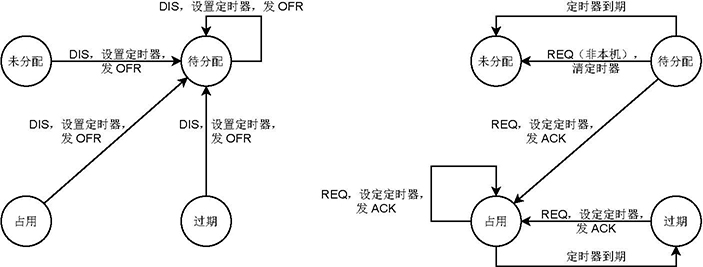
\includegraphics[width=0.95\textwidth]{image/22/3-p-1.jpg}
    % \caption{神经元 $v$ 变量随时间变化的曲线}
\end{figure}


\subsection*{输入格式}

输入的第一行包含用空格分隔的四个正整数和一个字符串,分别是:$N$、$T_{def}$、$T_{max}$、$T_{min}$ 和 $H$,保证 $T_{min} \le T_{def} \le T_{max}$。

输入的第二行是一个正整数 $n$,表示收到了 $n$ 个报文。

输入接下来有 $n$ 行,第 $(i+2)$ 行有空格分隔的正整数 $t_i$ 和约定格式的报文 $P_i$。表示收到的第 $i$ 个报文是在 $t_i$ 时刻收到的,报文内容是 $P_i$。保证 $t_i < t_{i+1}$。


\subsection*{输出格式}

输出有若干行,每行是一个约定格式的报文。依次输出 DHCP 服务器发送的报文。

\examplebox*{\lstinputlisting[frame=none]{data/22/3-1.in}}{\lstinputlisting[frame=none]{data/22/3-1.out}}

输入第一行,分别设置了 DHCP 的相关参数,并收到了 16 个报文。

第 1 个报文和第 2 个报文是客户端 a 正常请求地址,服务器为其分配了地址 1,相应地设置了过期时刻是 7(即当前时刻 2 加上默认过期时间 5)。

第 3 个报文不符合 Discover 报文的要求,不做任何处理。

第 4 个报文 b 发送的 Discover 报文虽然有 IP 地址 3,但是按照处理规则,这个字段被忽略,因此服务器返回 Offer 报文,过期时刻是 9。

第 5 个报文中,Request 报文不符合接收主机是 DHCP 服务器本机的要求,因此不做任何处理。

第 6 个报文是 b 发送的 Request 报文,其中设置了过期时刻是 12,没有超过最长过期时间,因此返回的 Ack 报文中过期时刻也是 12。

第 7 个报文中,过期时刻 11 小于最短过期时间,因此返回的过期时刻是 12。虽然此时为 a 分配的地址 1 过期,但是由于还有状态为未分配的地址 3,因此为 c 分配地址 3。第 8 个报文同理,为 c 分配的地址过期时刻是 13。

第 9、10 两个报文中,为 d 分配了地址 4,过期时刻是 20。

第 11 个报文中,a 请求重新获取此前为其分配的地址 1,虽然为其分配的地址过期,但是由于尚未分配给其它客户端,因此 DHCP 服务器可以直接为其重新分配该地址,并重新设置过期时刻为 20。

第 12 个报文中,c 请求延长其地址的过期时刻为 20。DHCP 正常向其回复 Ack 报文。

第 13、14 个报文中,e 试图请求地址。此时地址池中已经没有处于“未分配”状态的地址了,但是有此前分配给 b 的地址 2 的状态是“过期”,因此把该地址重新分配给 e。

第 15 个报文中,b 试图重新获取此前为其分配的地址 2,但是此时该地址已经被分配给 e,因此返回 Nak 报文。

第 16 个报文中,b 试图重新请求分配一个 IP 地址,但是此时地址池中已经没有可用的地址了,因此忽略该请求。

\examplebox*{\lstinputlisting[frame=none]{data/22/3-2.in}}{\lstinputlisting[frame=none]{data/22/3-2.out}}

在本样例中,DHCP 服务器一共收到了 6 个报文,处理情况如下:

第 1 个报文不是 DHCP 服务器需要处理的报文,因此不回复任何报文。

第 2 个报文中,b 请求分配 IP 地址,因此 DHCP 服务器将地址 1 分配给 b,此时,地址 1 进入待分配状态,DHCP 服务器向 b 发送 Offer 报文。

第 3 个报文中,b 发送的 REQ 报文是发给非本服务器的,因此需要将地址池中所有拥有者是 b 的待分配状态的地址修改为未分配。

第 4 个报文中,c 请求分配 IP 地址。由于地址 1 此时是未分配状态,因此将该地址分配给它,向它发送 Offer 报文,地址 1 进入待分配状态。

第 5、6 个报文中,d 请求分配 IP 地址。注意到在收到第 5 个报文时,已经是时刻 70,地址 1 的过期时刻已到,它的状态已经被修改为了未分配,因此 DHCP 服务器仍然将地址 1 分配给 d。

\subsection*{子任务}

对于 20\% 的数据,有 $N\le 200$,且 $n\le N$,且输入仅含 Discover 报文,且 $t < T_{min}$;

对于 50\% 的数据,有 $N\le 200$,且 $n\le N$,且 $t < T_{min}$,且报文的接收主机或为本机,或为 \*;

对于 70\% 的数据,有 $N\le 1000$,且 $n\le N$,且报文的接收主机或为本机,或为 \*;

对于 100\% 的数据,有 $N\le 10000$,且 $n\le 10000$,主机名的长度不超过 20,且 $t,T_{min},T_{default},T_{max}\le 10^9$,输入的报文格式符合题目要求,且数字不超过 $10^9$。